% Created by tikzDevice version 0.12.3 on 2019-09-26 18:31:10
% !TEX encoding = UTF-8 Unicode
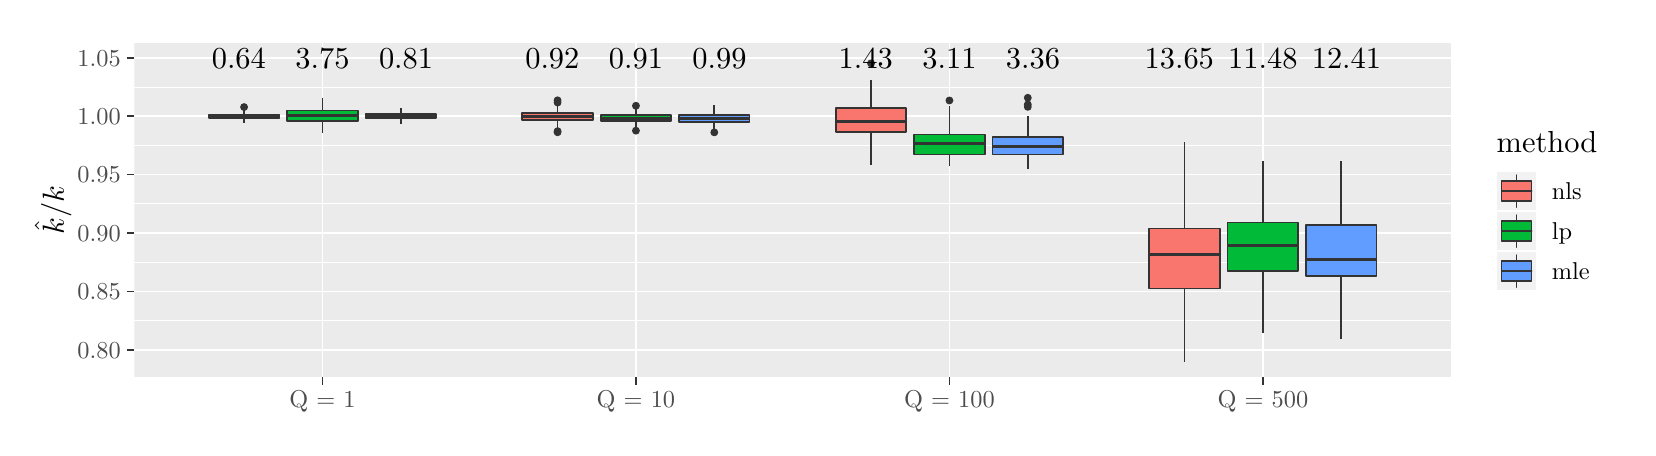
\begin{tikzpicture}[x=1pt,y=1pt]
\definecolor{fillColor}{RGB}{255,255,255}
\path[use as bounding box,fill=fillColor,fill opacity=0.00] (0,0) rectangle (578.16,144.54);
\begin{scope}
\path[clip] (  0.00,  0.00) rectangle (578.16,144.54);
\definecolor{drawColor}{RGB}{255,255,255}
\definecolor{fillColor}{RGB}{255,255,255}

\path[draw=drawColor,line width= 0.6pt,line join=round,line cap=round,fill=fillColor] (  0.00,  0.00) rectangle (578.16,144.54);
\end{scope}
\begin{scope}
\path[clip] ( 38.56, 18.22) rectangle (514.31,139.04);
\definecolor{fillColor}{gray}{0.92}

\path[fill=fillColor] ( 38.56, 18.22) rectangle (514.31,139.04);
\definecolor{drawColor}{RGB}{255,255,255}

\path[draw=drawColor,line width= 0.3pt,line join=round] ( 38.56, 38.69) --
	(514.31, 38.69);

\path[draw=drawColor,line width= 0.3pt,line join=round] ( 38.56, 59.80) --
	(514.31, 59.80);

\path[draw=drawColor,line width= 0.3pt,line join=round] ( 38.56, 80.91) --
	(514.31, 80.91);

\path[draw=drawColor,line width= 0.3pt,line join=round] ( 38.56,102.02) --
	(514.31,102.02);

\path[draw=drawColor,line width= 0.3pt,line join=round] ( 38.56,123.13) --
	(514.31,123.13);

\path[draw=drawColor,line width= 0.6pt,line join=round] ( 38.56, 28.13) --
	(514.31, 28.13);

\path[draw=drawColor,line width= 0.6pt,line join=round] ( 38.56, 49.24) --
	(514.31, 49.24);

\path[draw=drawColor,line width= 0.6pt,line join=round] ( 38.56, 70.35) --
	(514.31, 70.35);

\path[draw=drawColor,line width= 0.6pt,line join=round] ( 38.56, 91.46) --
	(514.31, 91.46);

\path[draw=drawColor,line width= 0.6pt,line join=round] ( 38.56,112.57) --
	(514.31,112.57);

\path[draw=drawColor,line width= 0.6pt,line join=round] ( 38.56,133.68) --
	(514.31,133.68);

\path[draw=drawColor,line width= 0.6pt,line join=round] (106.52, 18.22) --
	(106.52,139.04);

\path[draw=drawColor,line width= 0.6pt,line join=round] (219.79, 18.22) --
	(219.79,139.04);

\path[draw=drawColor,line width= 0.6pt,line join=round] (333.07, 18.22) --
	(333.07,139.04);

\path[draw=drawColor,line width= 0.6pt,line join=round] (446.34, 18.22) --
	(446.34,139.04);
\definecolor{drawColor}{gray}{0.20}
\definecolor{fillColor}{gray}{0.20}

\path[draw=drawColor,line width= 0.4pt,line join=round,line cap=round,fill=fillColor] ( 78.20,115.84) circle (  1.21);

\path[draw=drawColor,line width= 0.6pt,line join=round] ( 78.20,113.16) -- ( 78.20,114.96);

\path[draw=drawColor,line width= 0.6pt,line join=round] ( 78.20,111.95) -- ( 78.20,110.26);
\definecolor{fillColor}{RGB}{248,118,109}

\path[draw=drawColor,line width= 0.6pt,line join=round,line cap=round,fill=fillColor] ( 65.46,113.16) --
	( 65.46,111.95) --
	( 90.94,111.95) --
	( 90.94,113.16) --
	( 65.46,113.16) --
	cycle;

\path[draw=drawColor,line width= 1.1pt,line join=round] ( 65.46,112.53) -- ( 90.94,112.53);

\path[draw=drawColor,line width= 0.6pt,line join=round] (106.52,114.61) -- (106.52,119.28);

\path[draw=drawColor,line width= 0.6pt,line join=round] (106.52,110.92) -- (106.52,106.46);
\definecolor{fillColor}{RGB}{0,186,56}

\path[draw=drawColor,line width= 0.6pt,line join=round,line cap=round,fill=fillColor] ( 93.78,114.61) --
	( 93.78,110.92) --
	(119.26,110.92) --
	(119.26,114.61) --
	( 93.78,114.61) --
	cycle;

\path[draw=drawColor,line width= 1.1pt,line join=round] ( 93.78,112.63) -- (119.26,112.63);

\path[draw=drawColor,line width= 0.6pt,line join=round] (134.84,113.41) -- (134.84,115.64);

\path[draw=drawColor,line width= 0.6pt,line join=round] (134.84,111.90) -- (134.84,109.83);
\definecolor{fillColor}{RGB}{97,156,255}

\path[draw=drawColor,line width= 0.6pt,line join=round,line cap=round,fill=fillColor] (122.09,113.41) --
	(122.09,111.90) --
	(147.58,111.90) --
	(147.58,113.41) --
	(122.09,113.41) --
	cycle;

\path[draw=drawColor,line width= 1.1pt,line join=round] (122.09,112.45) -- (147.58,112.45);
\definecolor{fillColor}{gray}{0.20}

\path[draw=drawColor,line width= 0.4pt,line join=round,line cap=round,fill=fillColor] (191.48,107.14) circle (  1.21);

\path[draw=drawColor,line width= 0.4pt,line join=round,line cap=round,fill=fillColor] (191.48,117.48) circle (  1.21);

\path[draw=drawColor,line width= 0.4pt,line join=round,line cap=round,fill=fillColor] (191.48,106.74) circle (  1.21);

\path[draw=drawColor,line width= 0.4pt,line join=round,line cap=round,fill=fillColor] (191.48,118.29) circle (  1.21);

\path[draw=drawColor,line width= 0.6pt,line join=round] (191.48,113.73) -- (191.48,116.74);

\path[draw=drawColor,line width= 0.6pt,line join=round] (191.48,111.23) -- (191.48,108.12);
\definecolor{fillColor}{RGB}{248,118,109}

\path[draw=drawColor,line width= 0.6pt,line join=round,line cap=round,fill=fillColor] (178.73,113.73) --
	(178.73,111.23) --
	(204.22,111.23) --
	(204.22,113.73) --
	(178.73,113.73) --
	cycle;

\path[draw=drawColor,line width= 1.1pt,line join=round] (178.73,112.55) -- (204.22,112.55);
\definecolor{fillColor}{gray}{0.20}

\path[draw=drawColor,line width= 0.4pt,line join=round,line cap=round,fill=fillColor] (219.79,107.32) circle (  1.21);

\path[draw=drawColor,line width= 0.4pt,line join=round,line cap=round,fill=fillColor] (219.79,116.32) circle (  1.21);

\path[draw=drawColor,line width= 0.6pt,line join=round] (219.79,112.93) -- (219.79,115.54);

\path[draw=drawColor,line width= 0.6pt,line join=round] (219.79,110.73) -- (219.79,107.48);
\definecolor{fillColor}{RGB}{0,186,56}

\path[draw=drawColor,line width= 0.6pt,line join=round,line cap=round,fill=fillColor] (207.05,112.93) --
	(207.05,110.73) --
	(232.54,110.73) --
	(232.54,112.93) --
	(207.05,112.93) --
	cycle;

\path[draw=drawColor,line width= 1.1pt,line join=round] (207.05,111.80) -- (232.54,111.80);
\definecolor{fillColor}{gray}{0.20}

\path[draw=drawColor,line width= 0.4pt,line join=round,line cap=round,fill=fillColor] (248.11,106.71) circle (  1.21);

\path[draw=drawColor,line width= 0.6pt,line join=round] (248.11,112.92) -- (248.11,116.42);

\path[draw=drawColor,line width= 0.6pt,line join=round] (248.11,110.52) -- (248.11,106.99);
\definecolor{fillColor}{RGB}{97,156,255}

\path[draw=drawColor,line width= 0.6pt,line join=round,line cap=round,fill=fillColor] (235.37,112.92) --
	(235.37,110.52) --
	(260.86,110.52) --
	(260.86,112.92) --
	(235.37,112.92) --
	cycle;

\path[draw=drawColor,line width= 1.1pt,line join=round] (235.37,111.89) -- (260.86,111.89);
\definecolor{fillColor}{gray}{0.20}

\path[draw=drawColor,line width= 0.4pt,line join=round,line cap=round,fill=fillColor] (304.75,131.64) circle (  1.21);

\path[draw=drawColor,line width= 0.6pt,line join=round] (304.75,115.44) -- (304.75,125.75);

\path[draw=drawColor,line width= 0.6pt,line join=round] (304.75,106.91) -- (304.75, 94.74);
\definecolor{fillColor}{RGB}{248,118,109}

\path[draw=drawColor,line width= 0.6pt,line join=round,line cap=round,fill=fillColor] (292.01,115.44) --
	(292.01,106.91) --
	(317.49,106.91) --
	(317.49,115.44) --
	(292.01,115.44) --
	cycle;

\path[draw=drawColor,line width= 1.1pt,line join=round] (292.01,110.75) -- (317.49,110.75);
\definecolor{fillColor}{gray}{0.20}

\path[draw=drawColor,line width= 0.4pt,line join=round,line cap=round,fill=fillColor] (333.07,118.23) circle (  1.21);

\path[draw=drawColor,line width= 0.6pt,line join=round] (333.07,105.94) -- (333.07,116.09);

\path[draw=drawColor,line width= 0.6pt,line join=round] (333.07, 98.65) -- (333.07, 94.39);
\definecolor{fillColor}{RGB}{0,186,56}

\path[draw=drawColor,line width= 0.6pt,line join=round,line cap=round,fill=fillColor] (320.33,105.94) --
	(320.33, 98.65) --
	(345.81, 98.65) --
	(345.81,105.94) --
	(320.33,105.94) --
	cycle;

\path[draw=drawColor,line width= 1.1pt,line join=round] (320.33,102.71) -- (345.81,102.71);
\definecolor{fillColor}{gray}{0.20}

\path[draw=drawColor,line width= 0.4pt,line join=round,line cap=round,fill=fillColor] (361.39,115.92) circle (  1.21);

\path[draw=drawColor,line width= 0.4pt,line join=round,line cap=round,fill=fillColor] (361.39,116.80) circle (  1.21);

\path[draw=drawColor,line width= 0.4pt,line join=round,line cap=round,fill=fillColor] (361.39,119.21) circle (  1.21);

\path[draw=drawColor,line width= 0.6pt,line join=round] (361.39,104.95) -- (361.39,112.57);

\path[draw=drawColor,line width= 0.6pt,line join=round] (361.39, 98.75) -- (361.39, 93.57);
\definecolor{fillColor}{RGB}{97,156,255}

\path[draw=drawColor,line width= 0.6pt,line join=round,line cap=round,fill=fillColor] (348.64,104.95) --
	(348.64, 98.75) --
	(374.13, 98.75) --
	(374.13,104.95) --
	(348.64,104.95) --
	cycle;

\path[draw=drawColor,line width= 1.1pt,line join=round] (348.64,101.57) -- (374.13,101.57);

\path[draw=drawColor,line width= 0.6pt,line join=round] (418.02, 71.96) -- (418.02,103.06);

\path[draw=drawColor,line width= 0.6pt,line join=round] (418.02, 50.27) -- (418.02, 23.71);
\definecolor{fillColor}{RGB}{248,118,109}

\path[draw=drawColor,line width= 0.6pt,line join=round,line cap=round,fill=fillColor] (405.28, 71.96) --
	(405.28, 50.27) --
	(430.77, 50.27) --
	(430.77, 71.96) --
	(405.28, 71.96) --
	cycle;

\path[draw=drawColor,line width= 1.1pt,line join=round] (405.28, 62.65) -- (430.77, 62.65);

\path[draw=drawColor,line width= 0.6pt,line join=round] (446.34, 74.14) -- (446.34, 96.48);

\path[draw=drawColor,line width= 0.6pt,line join=round] (446.34, 56.68) -- (446.34, 34.03);
\definecolor{fillColor}{RGB}{0,186,56}

\path[draw=drawColor,line width= 0.6pt,line join=round,line cap=round,fill=fillColor] (433.60, 74.14) --
	(433.60, 56.68) --
	(459.09, 56.68) --
	(459.09, 74.14) --
	(433.60, 74.14) --
	cycle;

\path[draw=drawColor,line width= 1.1pt,line join=round] (433.60, 65.79) -- (459.09, 65.79);

\path[draw=drawColor,line width= 0.6pt,line join=round] (474.66, 73.22) -- (474.66, 96.48);

\path[draw=drawColor,line width= 0.6pt,line join=round] (474.66, 54.72) -- (474.66, 32.20);
\definecolor{fillColor}{RGB}{97,156,255}

\path[draw=drawColor,line width= 0.6pt,line join=round,line cap=round,fill=fillColor] (461.92, 73.22) --
	(461.92, 54.72) --
	(487.40, 54.72) --
	(487.40, 73.22) --
	(461.92, 73.22) --
	cycle;

\path[draw=drawColor,line width= 1.1pt,line join=round] (461.92, 60.83) -- (487.40, 60.83);
\definecolor{drawColor}{RGB}{0,0,0}

\node[text=drawColor,anchor=base,inner sep=0pt, outer sep=0pt, scale=  1.10] at (136.73,129.75) {0.81};

\node[text=drawColor,anchor=base,inner sep=0pt, outer sep=0pt, scale=  1.10] at (106.52,129.75) {3.75};

\node[text=drawColor,anchor=base,inner sep=0pt, outer sep=0pt, scale=  1.10] at ( 76.31,129.75) {0.64};

\node[text=drawColor,anchor=base,inner sep=0pt, outer sep=0pt, scale=  1.10] at (250.00,129.75) {0.99};

\node[text=drawColor,anchor=base,inner sep=0pt, outer sep=0pt, scale=  1.10] at (219.79,129.75) {0.91};

\node[text=drawColor,anchor=base,inner sep=0pt, outer sep=0pt, scale=  1.10] at (189.59,129.75) {0.92};

\node[text=drawColor,anchor=base,inner sep=0pt, outer sep=0pt, scale=  1.10] at (363.28,129.75) {3.36};

\node[text=drawColor,anchor=base,inner sep=0pt, outer sep=0pt, scale=  1.10] at (333.07,129.75) {3.11};

\node[text=drawColor,anchor=base,inner sep=0pt, outer sep=0pt, scale=  1.10] at (302.86,129.75) {1.43};

\node[text=drawColor,anchor=base,inner sep=0pt, outer sep=0pt, scale=  1.10] at (476.55,129.75) {12.41};

\node[text=drawColor,anchor=base,inner sep=0pt, outer sep=0pt, scale=  1.10] at (446.34,129.75) {11.48};

\node[text=drawColor,anchor=base,inner sep=0pt, outer sep=0pt, scale=  1.10] at (416.14,129.75) {13.65};
\end{scope}
\begin{scope}
\path[clip] (  0.00,  0.00) rectangle (578.16,144.54);
\definecolor{drawColor}{gray}{0.30}

\node[text=drawColor,anchor=base east,inner sep=0pt, outer sep=0pt, scale=  0.88] at ( 33.61, 25.10) {0.80};

\node[text=drawColor,anchor=base east,inner sep=0pt, outer sep=0pt, scale=  0.88] at ( 33.61, 46.21) {0.85};

\node[text=drawColor,anchor=base east,inner sep=0pt, outer sep=0pt, scale=  0.88] at ( 33.61, 67.32) {0.90};

\node[text=drawColor,anchor=base east,inner sep=0pt, outer sep=0pt, scale=  0.88] at ( 33.61, 88.43) {0.95};

\node[text=drawColor,anchor=base east,inner sep=0pt, outer sep=0pt, scale=  0.88] at ( 33.61,109.54) {1.00};

\node[text=drawColor,anchor=base east,inner sep=0pt, outer sep=0pt, scale=  0.88] at ( 33.61,130.65) {1.05};
\end{scope}
\begin{scope}
\path[clip] (  0.00,  0.00) rectangle (578.16,144.54);
\definecolor{drawColor}{gray}{0.20}

\path[draw=drawColor,line width= 0.6pt,line join=round] ( 35.81, 28.13) --
	( 38.56, 28.13);

\path[draw=drawColor,line width= 0.6pt,line join=round] ( 35.81, 49.24) --
	( 38.56, 49.24);

\path[draw=drawColor,line width= 0.6pt,line join=round] ( 35.81, 70.35) --
	( 38.56, 70.35);

\path[draw=drawColor,line width= 0.6pt,line join=round] ( 35.81, 91.46) --
	( 38.56, 91.46);

\path[draw=drawColor,line width= 0.6pt,line join=round] ( 35.81,112.57) --
	( 38.56,112.57);

\path[draw=drawColor,line width= 0.6pt,line join=round] ( 35.81,133.68) --
	( 38.56,133.68);
\end{scope}
\begin{scope}
\path[clip] (  0.00,  0.00) rectangle (578.16,144.54);
\definecolor{drawColor}{gray}{0.20}

\path[draw=drawColor,line width= 0.6pt,line join=round] (106.52, 15.47) --
	(106.52, 18.22);

\path[draw=drawColor,line width= 0.6pt,line join=round] (219.79, 15.47) --
	(219.79, 18.22);

\path[draw=drawColor,line width= 0.6pt,line join=round] (333.07, 15.47) --
	(333.07, 18.22);

\path[draw=drawColor,line width= 0.6pt,line join=round] (446.34, 15.47) --
	(446.34, 18.22);
\end{scope}
\begin{scope}
\path[clip] (  0.00,  0.00) rectangle (578.16,144.54);
\definecolor{drawColor}{gray}{0.30}

\node[text=drawColor,anchor=base,inner sep=0pt, outer sep=0pt, scale=  0.88] at (106.52,  7.21) {Q = 1};

\node[text=drawColor,anchor=base,inner sep=0pt, outer sep=0pt, scale=  0.88] at (219.79,  7.21) {Q = 10};

\node[text=drawColor,anchor=base,inner sep=0pt, outer sep=0pt, scale=  0.88] at (333.07,  7.21) {Q = 100};

\node[text=drawColor,anchor=base,inner sep=0pt, outer sep=0pt, scale=  0.88] at (446.34,  7.21) {Q = 500};
\end{scope}
\begin{scope}
\path[clip] (  0.00,  0.00) rectangle (578.16,144.54);
\definecolor{drawColor}{RGB}{0,0,0}

\node[text=drawColor,rotate= 90.00,anchor=base,inner sep=0pt, outer sep=0pt, scale=  1.10] at ( 13.08, 78.63) {$\hat{k}/k$};
\end{scope}
\begin{scope}
\path[clip] (  0.00,  0.00) rectangle (578.16,144.54);
\definecolor{fillColor}{RGB}{255,255,255}

\path[fill=fillColor] (525.31, 43.84) rectangle (572.66,113.42);
\end{scope}
\begin{scope}
\path[clip] (  0.00,  0.00) rectangle (578.16,144.54);
\definecolor{drawColor}{RGB}{0,0,0}

\node[text=drawColor,anchor=base west,inner sep=0pt, outer sep=0pt, scale=  1.10] at (530.81, 99.27) {method};
\end{scope}
\begin{scope}
\path[clip] (  0.00,  0.00) rectangle (578.16,144.54);
\definecolor{drawColor}{RGB}{255,255,255}
\definecolor{fillColor}{gray}{0.95}

\path[draw=drawColor,line width= 0.6pt,line join=round,line cap=round,fill=fillColor] (530.81, 78.25) rectangle (545.26, 92.70);
\end{scope}
\begin{scope}
\path[clip] (  0.00,  0.00) rectangle (578.16,144.54);
\definecolor{drawColor}{gray}{0.20}

\path[draw=drawColor,line width= 0.6pt,line join=round,line cap=round] (538.03, 79.70) --
	(538.03, 81.86);

\path[draw=drawColor,line width= 0.6pt,line join=round,line cap=round] (538.03, 89.09) --
	(538.03, 91.26);
\definecolor{fillColor}{RGB}{248,118,109}

\path[draw=drawColor,line width= 0.6pt,line join=round,line cap=round,fill=fillColor] (532.61, 81.86) rectangle (543.45, 89.09);

\path[draw=drawColor,line width= 0.6pt,line join=round,line cap=round] (532.61, 85.48) --
	(543.45, 85.48);
\end{scope}
\begin{scope}
\path[clip] (  0.00,  0.00) rectangle (578.16,144.54);
\definecolor{drawColor}{RGB}{255,255,255}
\definecolor{fillColor}{gray}{0.95}

\path[draw=drawColor,line width= 0.6pt,line join=round,line cap=round,fill=fillColor] (530.81, 63.80) rectangle (545.26, 78.25);
\end{scope}
\begin{scope}
\path[clip] (  0.00,  0.00) rectangle (578.16,144.54);
\definecolor{drawColor}{gray}{0.20}

\path[draw=drawColor,line width= 0.6pt,line join=round,line cap=round] (538.03, 65.24) --
	(538.03, 67.41);

\path[draw=drawColor,line width= 0.6pt,line join=round,line cap=round] (538.03, 74.64) --
	(538.03, 76.81);
\definecolor{fillColor}{RGB}{0,186,56}

\path[draw=drawColor,line width= 0.6pt,line join=round,line cap=round,fill=fillColor] (532.61, 67.41) rectangle (543.45, 74.64);

\path[draw=drawColor,line width= 0.6pt,line join=round,line cap=round] (532.61, 71.02) --
	(543.45, 71.02);
\end{scope}
\begin{scope}
\path[clip] (  0.00,  0.00) rectangle (578.16,144.54);
\definecolor{drawColor}{RGB}{255,255,255}
\definecolor{fillColor}{gray}{0.95}

\path[draw=drawColor,line width= 0.6pt,line join=round,line cap=round,fill=fillColor] (530.81, 49.34) rectangle (545.26, 63.80);
\end{scope}
\begin{scope}
\path[clip] (  0.00,  0.00) rectangle (578.16,144.54);
\definecolor{drawColor}{gray}{0.20}

\path[draw=drawColor,line width= 0.6pt,line join=round,line cap=round] (538.03, 50.79) --
	(538.03, 52.96);

\path[draw=drawColor,line width= 0.6pt,line join=round,line cap=round] (538.03, 60.18) --
	(538.03, 62.35);
\definecolor{fillColor}{RGB}{97,156,255}

\path[draw=drawColor,line width= 0.6pt,line join=round,line cap=round,fill=fillColor] (532.61, 52.96) rectangle (543.45, 60.18);

\path[draw=drawColor,line width= 0.6pt,line join=round,line cap=round] (532.61, 56.57) --
	(543.45, 56.57);
\end{scope}
\begin{scope}
\path[clip] (  0.00,  0.00) rectangle (578.16,144.54);
\definecolor{drawColor}{RGB}{0,0,0}

\node[text=drawColor,anchor=base west,inner sep=0pt, outer sep=0pt, scale=  0.88] at (550.76, 82.45) {nls};
\end{scope}
\begin{scope}
\path[clip] (  0.00,  0.00) rectangle (578.16,144.54);
\definecolor{drawColor}{RGB}{0,0,0}

\node[text=drawColor,anchor=base west,inner sep=0pt, outer sep=0pt, scale=  0.88] at (550.76, 67.99) {lp};
\end{scope}
\begin{scope}
\path[clip] (  0.00,  0.00) rectangle (578.16,144.54);
\definecolor{drawColor}{RGB}{0,0,0}

\node[text=drawColor,anchor=base west,inner sep=0pt, outer sep=0pt, scale=  0.88] at (550.76, 53.54) {mle};
\end{scope}
\end{tikzpicture}
